% don't remove the folling lines, and edit the defintion of \main if needed
\documentclass[../report.tex]{subfiles}
\providecommand{\main}{..}
\IfEq{\jobname}{\currfilebase}{\AtEndDocument{\biblio}}{}
% until here

\begin{document}
% this is the extra information to be used for the general sections.
\section{Dark matter and Dark sectors at Colliders}

\subsection{Overview}

Present and prospective future colliders offer a unique opportunity to create DM in the laboratory. 
%The most promising opportunities arise when DM is created through a BSM mediator or withing BSM models that include DM candidates.
%As far as the collider center of mass energy (CME) (partonic CME for hadron colliders)  is above twice the DM mass, a pair of DM particles could be directly produced at colliders.
DM can be searched for at colliders when produced directly in beam-beam collisions in association with other Standard Model particle/s, or in the decays of SM particles or yet undiscovered beyond the Standard Model states. 
%which then subsequently decay into SM particles and the DM. 
In all cases the DM signal will consist of significant missing transverse energy (in addition to what is accounted for by standard neutrinos) plus highly energetic SM objects (for example jet/s, a $Z$-boson, a Higgs boson or a photon), or more complex SM final states in case of cascade decays. A discussion of the discovery potential for a few  benchmark models used for dark matter searches at high-energy colliders, as well as the visible decays of the DM mediators, can be found in the BSM chapter of this briefing book. 
Moreover, thermally produced light DM particles  call for different types of light DS mediators that couple to the SM through portals (see Chapter~\ref{chap:bsm}). 
Summary plots of the complementarity among many different accelarator-based experiments are shown in Sect.~\ref{sec:BSM-FIPs}.

\subsection{Complementarity of high-energy collider results with Direct and Indirect Detection}
\label{subsec:complementarity_collider}



%What is missing according to Caterina:
%\begin{itemize}
       % \item if needed, one can shorten the description of the Higgs portal model to just have the references there, I transferred it pretty much verbatim from the BSM PPG chapter (ran out of time today...)
       % \item short sentence/paragraph on running effects for conversion (if we converge with the discussion with Marcela);
       % \item Caveats on plots: use of simplified models limiting factor, EFT for Higgs to invisible model, collider curves are also bounded from above (cite Beacom);
      % \item indirect detection plots and discussion. (JRM I added this)
       % \item a final sentence saying that our ignorance of DM requires looking for closer collaboration with astrophysics, so we should seek more synergies (but maybe it does not belong here)
%        \end{itemize}
%}

%As shown in Fig.~\ref{fig:complementarity}, colliders, direct detection and indirect detection play complementary roles in searching for WIMP dark matter that interacts with SM particles. 

%\begin{figure}[htb!]
    %\centering
    %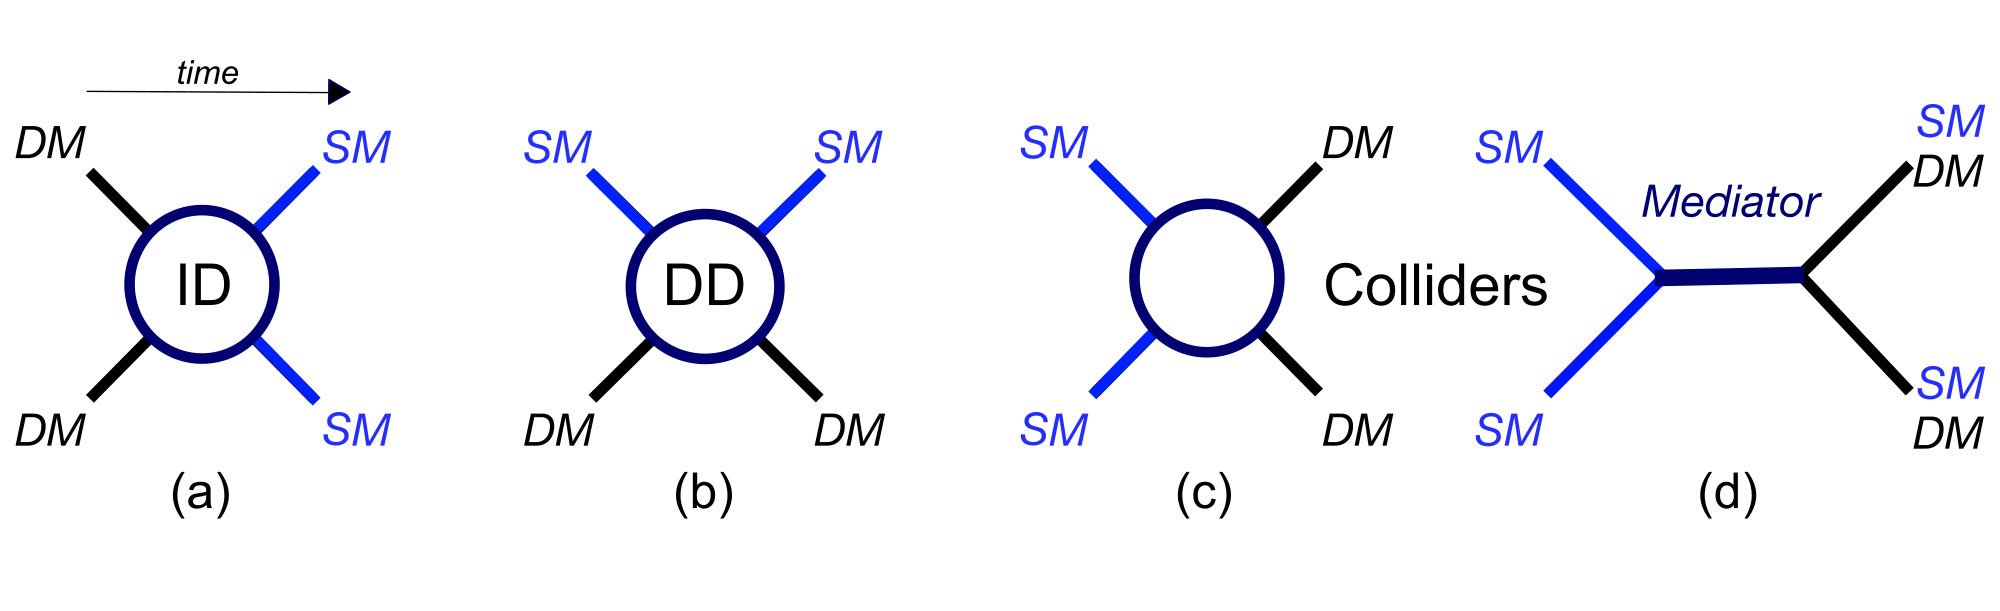
\includegraphics[width=\textwidth]{Darkmatter/section2/img/EFTSimplifiedModels.png}
   % \caption{Schematic illustration of the complementarity between colliders, direct detection and indirect detection for WIMP dark matter searches.}
   % \label{fig:complementarity}
%\end{figure}
    
%Fig.~\label{fig:complementarity} (a) shows DM particles annihilating to SM particles, as sought by space-based ID experiments. Fig.~\label{fig:complementarity} (b) shows the scattering of cosmic DM and SM particles in DD experiments.  Fig.~\label{fig:complementarity} (c) shows the production of DM particles from SM particle collisions at colliders, while Fig.~\label{fig:complementarity} (d) shows again pair production of DM as in Fig.~\label{fig:complementarity} (c), but in this case the interaction occurs through a mediator particle between DM and SM particles. 
%From this picture, it follows that DD and ID experiments are able to detect relic DM and are needed to confirm that an invisible particle discovered at colliders is stable on the timescale of the lifetime of the universe. A joint observation of consistent new phenomena at colliders, such as visible decays of a mediator particle between SM and DM, would shed light on the nature of this interaction.  

%This complementarity can be realized if the sensitivity of DD, ID and collider experiments is comparable, leading to a joint observation, thus confirming a dark matter discovery. 

The discovery of DM at direct and indirect detection experiments is necessary to ascertain the cosmological connection of a collider discovery, which in turn could provide information on the nature of the DM-SM interaction. 
Collider results make no assumptions on the thermal history of the dark matter candidate that is produced via the mediator particle considered as benchmark. In some regions of the parameter space covered by collider searches, a non-standard cosmology is needed to achieve the observed relic density.

The comparison of sensitivities across direct detection, indirect detection and collider experiments is possible within a given theoretical framework, and strongly depends on the choices of model and parameters. 
These comparisons nevertheless give an idea of the potential parameter space for a DM discovery if DM is realized in one of those example models. 

Firstly, this section discusses the complementarity between the collider sensitivity to Wino and Higgsino, as shown in Chapter~\ref{chap:bsm}, and the indirect detection projection for the same scenarios.
The comparison of direct detection and collider sensitivity for a Higgs portal model~\cite{Patt:2006fw,Djouadi:2011aa} is then shown, considering the results of the Higgs decays into invisible particles from Chapter~\ref{chap:ew}. Finally, the scalar benchmark model that has been discussed in Chapter~\ref{chap:bsm} is considered for comparison of colliders and direct detection experiments,  and a version of the same model with pseudoscalar couplings is used for comparison of colliders and indirect detection experiments.

\subsubsection*{Wino and Higgsino}

% indirect detection complementarity paragraph
The complementarity of collider and indirect detection searches within the Wino/Higgsino dark matter model is most evident at relatively high mass (see Fig.~\ref{fig:ID}). Above a DM mass of $\sim$ 0.5--1 TeV, ID provides strong constraints on dark matter annihilation, almost reaching the thermal cross-section~\cite{Abdallah:2016ygi}, via observations of the inner Galaxy with the H.E.S.S.~Cherenkov Telescope. Pure Wino dark matter with a mass around 2.9 TeV~\cite{Beneke:2016ync}, which would account for all of dark matter, is constrained by these searches, as well as searches for $\gamma\gamma$ final states, if the dark matter distribution at our Galactic center has a cusp-like profile~\cite{Cohen2013-ah, Cabrera-Catalan2015-os, Hryczuk2019-mv, Rinchiuso:2018ajn}.   However, if the distribution is more cored, the constraints become weaker. As shown in Chapter~\ref{chap:bsm}, Wino dark matter can also be probed with the FCC-hh~\cite{CidVidal:2018eel} and LE-FCC, while slightly lighter Wino-like dark matter would be already accessible for HE-LHC~\cite{CidVidal:2018eel} and CLIC$_{3000}$~\cite{deBlas:2018mhx}.
The future Cherenkov Telescope Array (CTA) will improve on current H.E.S.S.~constraints by another order of magnitude~\cite{Drlica-Wagner2019-nr, Carr2016-vl, Silverwood2015-ff}.  In the case of a discovery, the combination of CTA and collider results would allow to determine the dark matter distribution at the galactic center, with important implications for the formation history and evolution of galaxies.  CTA will be furthermore sensitive to Higgsino dark matter with a mass about $1.1$ TeV~\cite{Cabrera-Catalan2015-os, Krall:2017xij, Hryczuk2019-mv}, which is also a target of the FCC-hh~\cite{CidVidal:2018eel} and CLIC$_{3000}$~\cite{deBlas:2018mhx} as shown in Chapter~\ref{chap:bsm}. Interestingly, the cross section of many of these models would be lower than the neutrino background for direct searches, emphasizing the need for different experimental approaches.

\subsubsection*{Higgs portal, scalar and pseudoscalar mediator models}

\begin{figure}[!htbp]
    \centering
    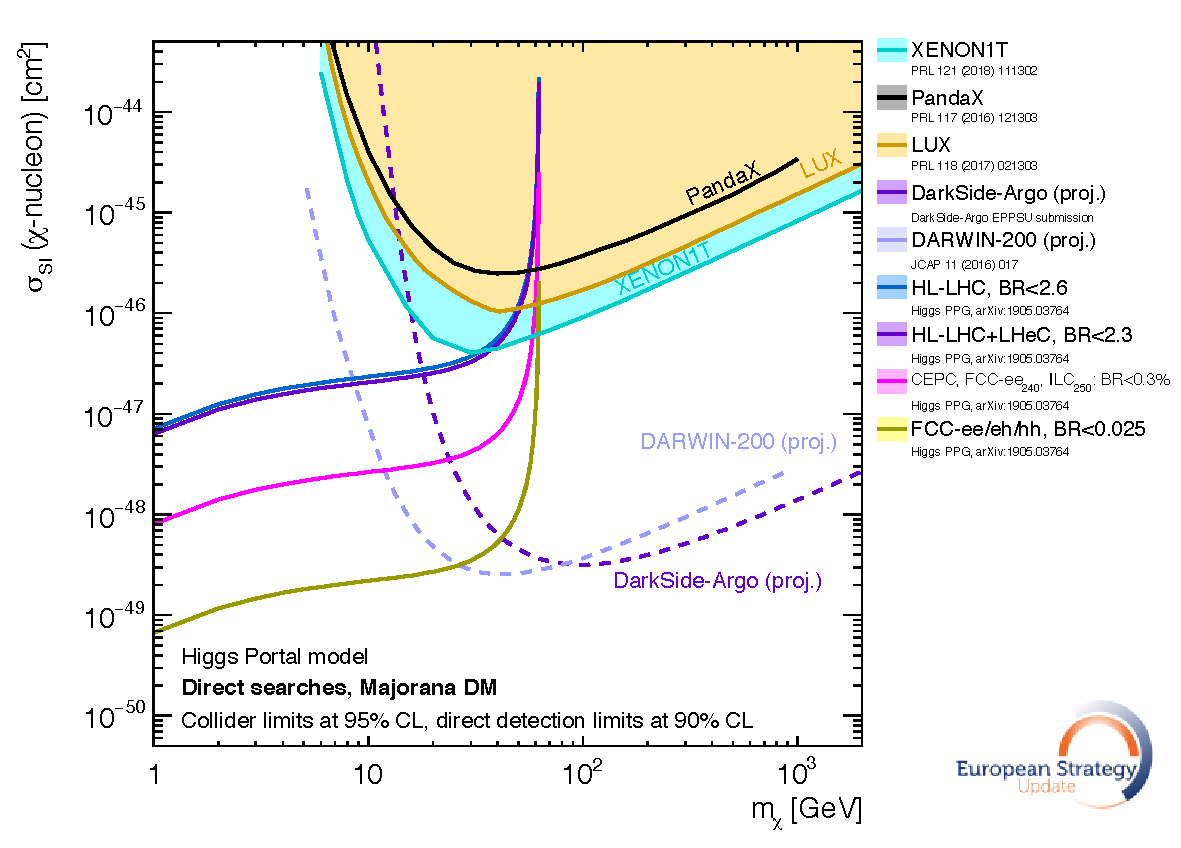
\includegraphics[width=0.78\textwidth]{Darkmatter/section2/img/DMCombinationDD_12May19_Internal_V1SInucleonMajorana}\\
    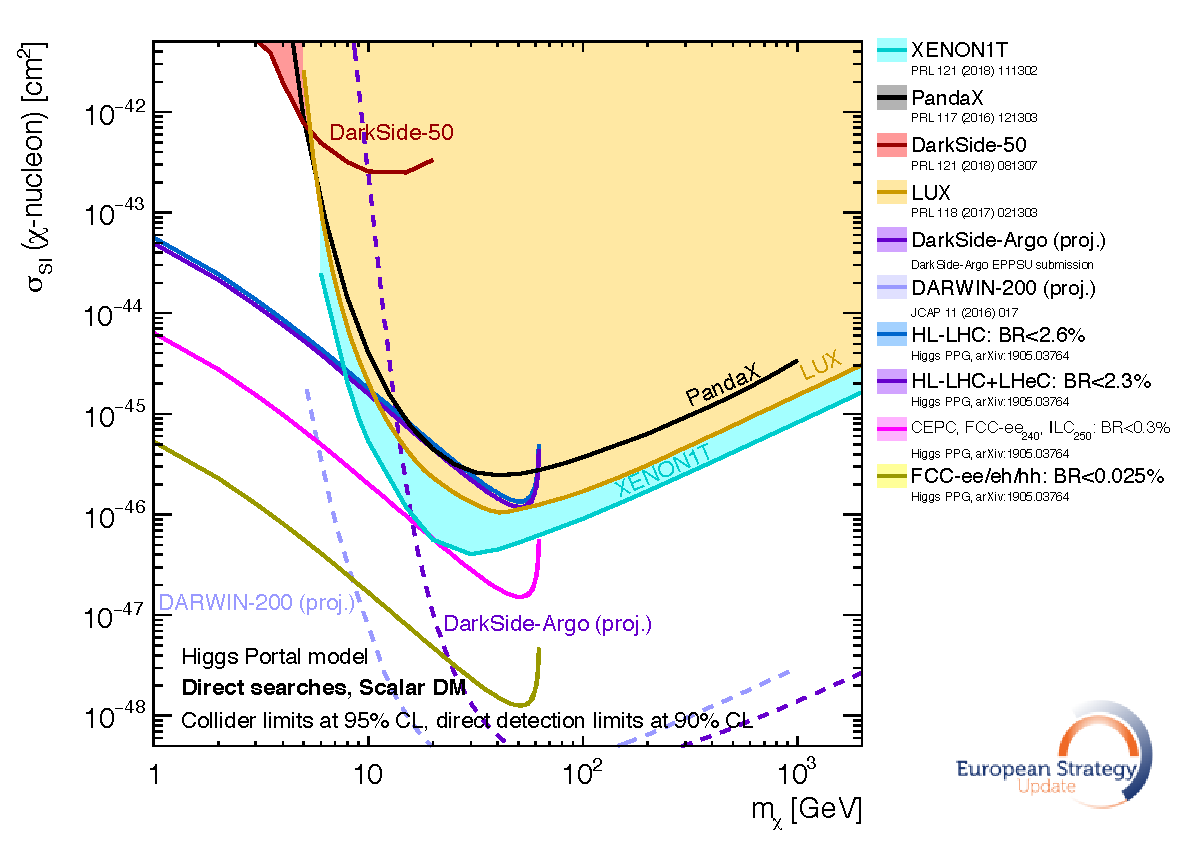
\includegraphics[width=0.78\textwidth]{Darkmatter/section2/img/DMCombinationDD_12May19_Internal_V1SInucleonScalar}
    \caption{Comparison of projected limits from future colliders (direct searches for invisible decays of the Higgs boson) with constraints from current and future direct detection experiments on the spin-independent WIMP--nucleon scattering cross-section for a simplified model with the Higgs boson decaying to invisible  (DM) particles, either Majorana (top) or scalar (bottom). Collider limits are shown at 95\% CL and direct detection limits at 90\% CL. 
    %The comparison is valid solely in the context of this model. 
    LHC searches and direct detection experiments exclude the areas above the curves. }
    \label{fig:Higgs_CollidersDD}
\end{figure}

Direct detection reach and future hadron collider reach for searches for invisible decays of the Higgs\footnote{Results from fits in the kappa-framework lead to similar conclusions.} are shown in Fig.~\ref{fig:Higgs_CollidersDD}, within the context of a Higgs portal model~\cite{Patt:2006fw,Djouadi:2011aa}. Collider results from Chapter~\ref{chap:ew} are translated to the nucleon-DM scattering plane using the procedure and factors in~\cite{Fox:2011pm, Hoferichter:2017olk}. 
The dark matter candidates considered as an example in these Higgs Portal benchmarks are either a scalar, or a Majorana fermion.

\begin{figure}[!htbp]
    \centering
          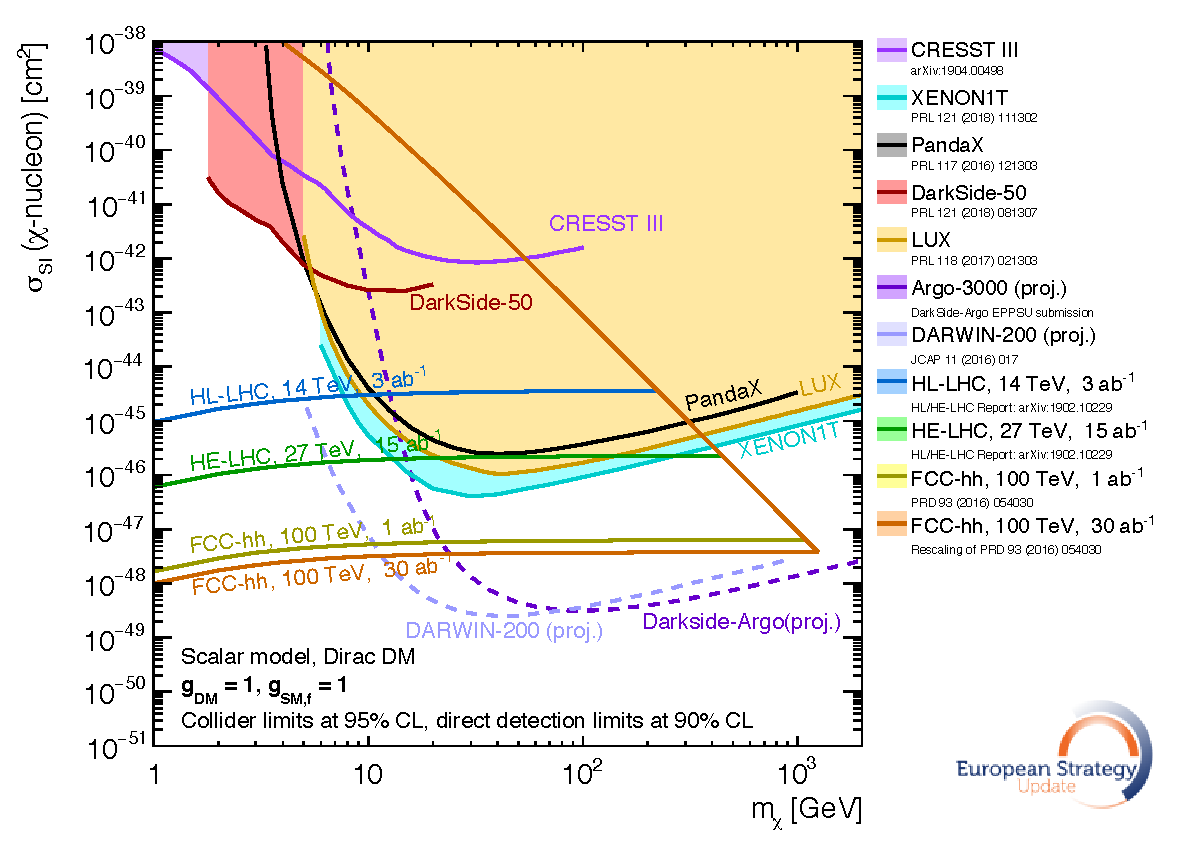
\includegraphics[width=0.78\textwidth]{Darkmatter/section2/img/DMCombinationDD_12May19_Internal_V1SInucleon}
        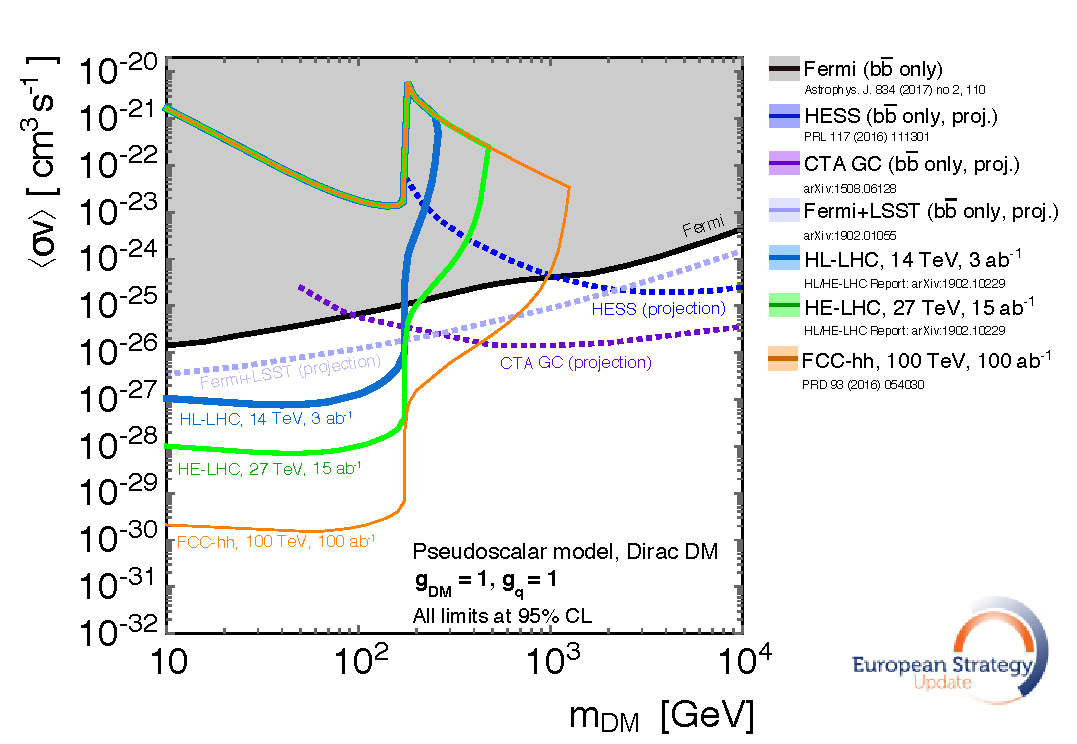
\includegraphics[width=0.78\textwidth]{Darkmatter/section2/img/ID_Formatted_allChannels}
    \caption{Top: Comparison of projected limits from future colliders with constraints from current and future direct detection experiments on the spin-independent WIMP--nucleon scattering cross-section in the context of a simplified model where a pseudoscalar particle with unit couplings mediates the interaction between SM fermions and Dirac fermionic DM. 
    LHC searches and direct detection experiments exclude the areas within the curves.
    Collider limits are shown at 95\% CL and direct detection limits at 90\% CL. 
    %The comparison is valid solely in the context of this model, assuming a mediator width fixed by the dark matter mass and the coupling values highlighted in each figure. 
    Bottom: comparison of a selection of projected limits from future colliders with constraints from current and future indirect detection experiments in the context of a simplified model where a pseudoscalar particle with unit couplings mediates the interaction between SM fermions and Dirac fermionic DM. All limits are shown at 95\% CL. }
    \label{fig:Scalar_CollidersDD}
\end{figure}

The comparison of the reach of DD, ID and future hadron colliders for the benchmark models of a scalar or pseudoscalar mediator decaying into Dirac DM use the procedure in~\cite{Boveia:2016mrp}, with the coupling choices made in Chapter [PPG BSM]. The results are shown in Figures~\ref{fig:Scalar_CollidersDD}. 
For the ID plot, the procedure in~\cite{Boveia:2016mrp} maps a velocity-averaged annihilation cross-section to multiple values of LHC mediator mass -- DM mass pairs.
Fig.~\ref{fig:Scalar_CollidersDD} considers that if a mapped velocity-averaged annihilation cross-section value is obtained from a mediator mass -- DM mass pair reachable by the LHC, that cross-section value is considered within LHC reach. 
Such a procedure highlights the potential of a 
the situation where a hint for invisible particles at colliders can guide ID searches and vice versa. 
The bounds from indirect detection experiment shown in Fig.~\ref{fig:Scalar_CollidersDD} only consider annihilation into b-quarks, while collider plots consider all channels. A full treatment would involve the calculation described in \cite{Carpenter:2016thc}. 

% direct detection complementarity paragraph
%Complementarity of direct detection and collider searches is most evident at high dark matter masses for scalar dark matter.  
From Figs.~\ref{fig:Higgs_CollidersDD} and \ref{fig:Scalar_CollidersDD} (top), one can observe that above $\sim$10 GeV DM mass, next-decade direct detection experiments are more sensitive than future colliders to DM signals. Future collider experiment, instead, are well  suited to explore models with mediators decaying to lighter DM candidates as well as reaching DM masses up to a TeV from the decays of multi-TeV-mass mediators.
%A 100 TeV hadron collider is well placed to produce DM particles with a mass range spanning more than a TeV from the decay of multi-TeV-mass mediators, translating to the reach shown in Fig.~\ref{fig:Scalar_CollidersDD}. 
From Fig.~\ref{fig:Scalar_CollidersDD} (bottom), it follows that collider searches have better sensitivity for DM masses below the top mass, while ID searches are more powerful for higher DM masses.  

Notably, it is in the intermediate DM mass range (roughly between 10 GeV and 1 TeV for the scalar/pseudoscalar cases, and between 10 GeV and half the Higgs mass for the Higgs portal models considered) that the combination of future high energy colliders, direct detection and indirect detection programs will complement each other and shed light into the nature of a dark matter candidate discovered in the next decades. 

%% CW:
% - beam dump experiments: nuMSM and sterile neutrino dark matter

\end{document}

